\documentclass{article}
\usepackage{caption}
\usepackage{subcaption}
\usepackage{graphicx}
\usepackage{tikz}
\usepackage{tikzsymbols}
\usetikzlibrary{calc}
\usepackage{float}
\usepackage{pdflscape}
\usepackage{geometry}
\geometry{a4paper, landscape, margin=1cm}
\pagestyle{empty}

\def\centerarc[#1](#2)(#3:#4:#5){\draw[#1] ($(#2)+({#5*cos(#3)},{#5*sin(#3)})$) arc (#3:#4:#5);}

\begin{document}
	\centering
	\begin{figure}[H]
			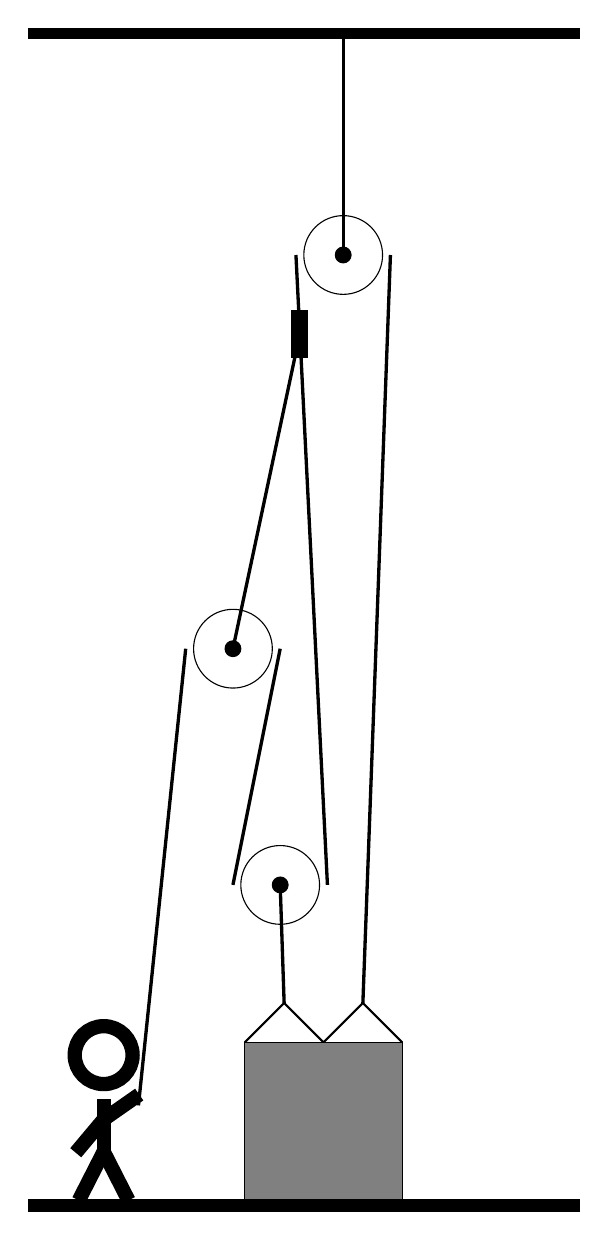
\begin{tikzpicture}
				%%%%% START %%%%%
								
				\draw[fill=black] (-2, 11.75) rectangle (5, 11.88);
				
				\draw (0.6, 4) circle (0.5);
				\draw[fill=black] (0.6, 4) circle (0.1);
				
				\draw (1.2, 1) circle (0.5);
				\draw[fill=black] (1.2, 1) circle (0.1);
				
				\draw (2, 9) circle (0.5);
				\draw[fill=black] (2, 9) circle (0.1);
				\draw[very thick] (2, 9) -- (2, 11.75);
				
				\draw[thick]  (0.75, -1) -- (1.25, -0.5) -- (1.75, -1) -- (2.25, -0.5) -- (2.75, -1);
				\draw[fill=black!50] (0.75, -1) rectangle (2.75, -3);
				
				\draw[very thick] (-0.6, -1.8) -- (0.0, 4);
				\draw[very thick] (0.6, 4) -- (1.45, 8);
				\draw[fill=black] (1.35, 7.7) rectangle (1.55, 8.3);
				\centerarc[very thick](0.6, 4)(0:180:0.6);
				\draw[very thick] (1.2, 4) -- (0.6, 1);
				\centerarc[very thick](1.2, 1)(180:360:0.6);
				\draw[very thick](1.2, 1) -- (1.25, -0.5);
				\draw[very thick] (1.8, 1) -- (1.4, 9);
				\centerarc[very thick](2, 9)(0:180:0.6);
				\draw[very thick] (2.6, 9) -- (2.25, -0.5);
				
				\node at (-1, -1.9) {\Strichmaxerl[10][50][35]};
				
				\draw[fill=black] (-2, -3) rectangle (5, -3.15);
				%%%%% END %%%%%
			\end{tikzpicture}
	\end{figure}	
\end{document}